\chapter{Team 6 Agent Design}\label{team_6_agent_design}

\section{Overview}

In this chapter, we present the technical formulation and results of the Team 6 agent. This chapter is divided into \ToDo{3 parts} and is structured as follows: 
\begin{enumerate}
    \item Introduce the underlying social motives that our agents can follow in \Cref{social_motives}, which define the way our agents utilise common pool resources \Cref{food_consumption} and interact with one-another. 
    \item Explain how the social motives are linked to communication and formation of a social network in \Cref{communication}
    
    \item Illustrate a set of experimental results \Cref{simulation_results}. 
\end{enumerate}

Ultimately, we propose that this agent accurately parallels aspects of human nature through its capability to undergo behavioural change and formulate social connections with trust.

%%%%%%%%%
%%%%%%%%% AGENT SPECIFICATION
%%%%%%%%%%%%%%%%%%%%%%%%%%%%%%%%%%%%%%%%%%%%%%%%%

\section{Specification of Agent Design}

All agents \textit{i} $\in$ \textit{A} are implemented as a data structure, such that all agents contain sufficient parameterisation to participate in the various communication methods \textit{c} $\in$ \textit{C}, resulting in a set of interactions defined by I = $< \mathit{A, C} >$. Each agent inherits from the \textit{baseAgent} structure, before inheriting the fields contained in table \ref{tab:agentStruct}. We note only the most relevant fields for quantifying the agent have been included.

\begin{table}[H]
  \begin{center}
    \begin{tabular}{c|c}
      \textbf{Parameter} & \textbf{Range}\\
      \hline
      BaseBehaviour & \textit{N} $\in$ [0,10]\\
      Stubbornness & \textit{N} $\in$ [0,1]\\
      MaxBehaviourSwing & \textit{N} $\in$ [0,10]\\
      ParamWeights & \{ HPWeight:\textit{N}, FloorWeight:\textit{N} \} \\
      FloorDiscount & \textit{N} $\in$ [0,1]\\
      MaxBehaviour & \textit{N} = 10\\
      PrevFoodDiscount & \textit{N} $\in$ [0,1]\\
      MaxTrust & \textit{N} = 25\\
    \end{tabular}
    \caption{Parameters held in the \textit{Config} data structure}
    \label{tab:agentConfig}
\end{center}   
\end{table}


\begin{table}[H]
  \begin{center}
    \begin{tabular}{c|c}
      \textbf{Parameter} & \textbf{Range}\\
      \hline
      BaseAgentRef & *baseAgent\\
      Config & config\{\} (see \Cref{tab:agentConfig})\\
      CurrBehaviour & \textit{N}\\
      MaxFloorGuess & \textit{N}\\
      AverageFoodIntake & \textit{N}\\
      ShortTermMemory & [\textit{N}]\\
      LongTermMemory & [\textit{N}]\\
      ProposedTreaties & [\textit{Treaty}] \\
      TrustTeams & map\{ \textit{UUID}, \textit{N} \} \\
      Neighbours & \{ above:\textit{UUID}, below:\textit{UUID} \} \\
    \end{tabular}
    \caption{Parameters held in the \textit{Agent} data structure}
    \label{tab:agentStruct}
\end{center}   
\end{table}


%%%%%%%%%
%%%%%%%%% SOCIAL MOTIVES
%%%%%%%%%%%%%%%%%%%%%%%%%%%%%%%%%%%%%%%%%%%%%%%%%
\section{Social Motives}\label{social_motives}
%%
%% Theoretical Framework
%%
\subsection{Social Motives}
The initial basic concept revolves around the four possible social motives that this agent can have based on different principles, practices, or characteristics. These behaviour types are: 

\begin{itemize}
    \item \textbf{Altruism:} The disinterested and selfless concern for the well-being of others. An altruist then acts in a way that purely benefits others, even if it means harming themselves.
    \item \textbf{Collectivism:} The practice or principle of giving a group priority over each individual in it. A collectivist then acts in a way that benefits the group, themselves included, over purely the individual.
    \item \textbf{Selfishness:} Being concerned excessively or exclusively with oneself. A selfish agent will act in a way to satisfy themselves, but not necessarily with intent to harm the other agents.
    \item \textbf{Narcissism:} An excessive interest or admiration of oneself. A narcissistic agent will act in a way that purely benefits themselves, even to the extent of harming others.
\end{itemize}


\subsection{Changing Social Motives}
Placing an agent into one of these fixed categories for the entire duration of the game would be limiting and unrealistic. This led to the addition of the first layer of complexity. Given that an agent may be initially assigned a social motive, it should be plausible for the agent to change their social motive based on their experience. This concept brings forth the interesting duality of ``nature vs nurture''. One could also think about this in terms of “genotype vs phenotype”. For example, an agent may “naturally”, “genetically”, be born a collectivist but may be incentivised to change its values and act selfishly if it becomes desperate due to a lack of food. In this environment, the decided upon influential factors in changing an agent’s social motive and behaviour, include current HP (lower HP means more likely for an agent to act selfishly/narcissistically), and current floor (lower floor means the agent will be worried about food supply, thus may be incentivised to act selfishly).

\subsection{Willingness to Change}
Although the above encapsulates an essential human characteristic, the ability to change, an important element of the human nature, its willingness to change, is missing. Through this next layer of complexity, we attempt to quantify how resistant an agent is to altering their behaviour. This concept brings forth more freedom for modelling different human characteristics and realistic situations. For example, it is now possible to distinguish between an agent who is initially an altruist, but then may become selfish as the supply of food diminishes, and an agent who is a “true altruist”, who will stick to their values for the duration of the game, retaining the same social motive throughout. Similarly, this is extended to the distinction between a true narcissist who never changes, and a narcissist who may, during the game, witness others suffering whilst it itself has an abundance of food, and therefore steer towards a more collectivist behaviour. %(Narcissistic personality disorder is not curable (though it is treatable) but I’m happy to ignore this for now for the purposes of the report : ))

\subsection{Bounding Change}
The agent we propose is currently assigned an initial social motive and is then able to change throughout the duration of the game. The ease with which it changes is also quantified through its willingness to change. This brought forth the possibility that even though an agent might be stubborn/resistant to change, it is still, given a long enough period, able to go from a narcissist to an altruist. This, considered to be unrealistic, lead to the final addition of complexity concerning the prevention of extreme changes in social motive. Prior to the start of the game, we define how far an agent can steer away from their “genetic” or “natural” initial state.

%%
%% Mathematical Formulation
%%
\subsection{Mathematical Formulation}\label{mathematical_formulation}
In order to implement our agent's behaviour, we present a mathematical formulation and its implementation for each of the steps introduced above.

\subsubsection{Define Social Motives}

Social motives can be defined in a spectrum, with one end corresponding to pure altruism and the other end corresponding to pure narcissism. All agents fall on some point on this spectrum of social motives. This is represented as a continuous value between 0.0 and 10.0 that shows where an agent lies in the social motive spectrum. Using a continuous rather than discrete variable for the social motive allows for more expressiveness. For example, two agents may both be referred to as collectivists, but one may be significantly closer to turning selfish than the other. A number closer to 0.0 corresponds to altruistic behaviours, and a number closer to 10.0 corresponds to narcissistic behaviour. The boundaries for the 4 distinct social motives are shown in Figure \ref{fig:socialMotives}. The initial “natural” state of a given agent is also shown and is labelled \texttt{baseBehaviour}. 

The current social motive of the agent is also shown and is labelled $\texttt{currentBehaviour}$. To begin, we set $\texttt{currentBehaviour} =\texttt{baseBehaviour}$.

\begin{figure}[htb]
    \centering
    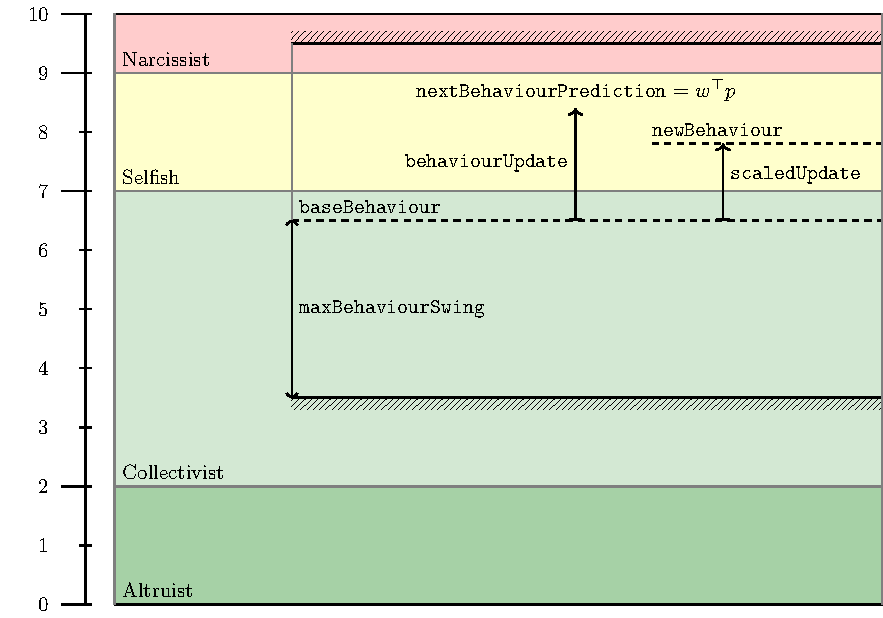
\includegraphics[width=0.9\textwidth]{008_team_6_agent_design/SOMAS_social_motives.pdf}
    \caption{Social motive spectrum and update procedure. \ToDo{Add a few additional comments to understand the pictures without having to read to whole text - this is what reviewers typically do at first.}}
    \label{fig:socialMotives}
\end{figure}

\subsubsection{Changing Social Motives}

Changing an agent's social motive based on certain factors can be represented as a weighted sum of these factors. In this case, where the related parameters are the current HP value and the current floor, the weighted sum can be achieved by defining a parameters vector $p$ and a weights vector $w$. The weighted sum is then given by the product $w^\top{}p$. These are shown below:


\begin{equation}
    \begin{gathered}
    p = [currentHP, currentFloor],\quad w=[weightHP, weightFloor] \\ 
    w^\top{}p = weightHP*currentHP + weightFloor*currentFloor
    \end{gathered}
\end{equation}





\begin{center}
    \textit{\textbf{********** Matt's adaptive weights should be here **********}} \\
    \textit{\textbf{********** Maybe also HP / Floor utility function **********}}
\end{center}
Based on how social motive has been mapped between 0.0 and 10.0, a lower floor (\emph{i.e.,} greater floor number) and a lower HP (\emph{i.e.,} smaller HP value) should push the social motive variable to be higher. The weights should then be chosen to reflect these correlations, along with any necessary feature transformations applied to these factors.



This weighted sum represents the prediction of our next social motive, titled \texttt{nextBehaviourPrediction} in the Figure below. We therefore calculate:

\begin{equation}
    behaviourUpdate = nextBehaviourPrediction - currentBehaviour
\end{equation}


For the first iteration $currentBehaviour=baseBehaviour$ as presented in \Cref{fig:socialMotives}.

\subsubsection{Willingness to Change}

To represent the willingness of an agent to change its social motive, an additional parameter, labelled as $stubbornness$, is introduced and instantiated as a number between 0.0 and 1.0. This number (or, precisely, one minus this number) is multiplied with the behaviour update. This operation is similar to a step-size, and it reflects how easy it is for the social motive to change. We therefore calculate the $scaledUpdate$ and $newBehaviour$ as shown below.


\begin{equation}
    \begin{gathered}
    scaledUpdate = behaviourUpdate *(1-stubbornness) \\ 
    newBehaviour = currentBehaviour + scaledUpdate
    \end{gathered}
\end{equation}


Again, $currentBehaviour=baseBehaviour$ for the first iteration.

\subsubsection{Bounding Change}

Bounding social motive change is modelled through the addition of the parameter \textit{maxBehaviourSwing}. This parameter allows us to define the maximum and minimum values of the allowed social motive for an agent, thus defining a range:

\vspace{0.2cm}
\begin{equation}
    \begin{gathered}
    max=baseBehaviour+maxBehaviourSwing  \\ 
    \texttt{min}=\texttt{baseBehaviour}-\texttt{maxBehaviourSwing }
    \end{gathered}
\end{equation}
\vspace{0.2cm}

If the change as defined in Step 3 above results in a \textit{newBehaviour} outside this range, then this is automatically capped off at the edges. This obviously also holds for the spectrum edges $\{0,10\}$.


%%%%%%%%%%
%%%%%%%%%% TRUST
%%%%%%%%%%%%%%%%%%%%%%%%%%%%%%%%%%%%%%%%%%%%%%%%%%%%%%
\section{Trust}

\subsection{Background}

With treaties offering a notion of socially accepted institutional power, the formation of treaties must be handled carefully, so as not to disadvantage the agents who engage in them. For this reason, a social network must be constructed to offer a heuristic for joining into these agreements. 

Trust serves as ``an important role formation of coalitions in social networks and in determining how high value of information flows through the network'' \cite{trustEEE}, with Ostrom futhermore supporting that ``trust is an essential social lubricant'' \cite{ostrom2003trust}. Ostrom further asserts that trust ``affects the willingness to cooperate'' \cite{ostrom2003trust} and ``enhances cooperation in social-dilemma experiments'' \cite{ostrom2003trust}, providing clear reasoning that trust is an effective parameter to introduce to the agent structure.

Finally, it is through this introduction of trust that we demonstrate the assertion from Adali's work \cite{trustEEE} that trust facilitates `` communication behaviors which are statistically different from random communications.''

\subsection{Initialisation}
The agent takes a simple algorithmic approach to formulating a social network; firstly, the ID of the neighbouring agents is determined through message passing, this ID is mapped to an initial trust value and the trust value is continually updated through subsequent social interactions. 

This agent implementation offers different initialised trust values based on the social motive, using the general notion that the more narcissistic an agent is, the less likely it is to have an initial positive opinion of their neighbours. 

For this reason, we give a maximal range of trust from -25 to +25 with the initialisations as follows:

\begin{itemize}
    \item Narcissist: -5
    \item Selfish: 0
    \item Collectivist: +5
    \item Altruist: +10
\end{itemize}

\subsection{Causes for Trust Update}

It is through continuous social interaction in the tower that agents will be able to form opinions of the other agents. For this agent, there is a specific set of interactions that will result in a opportunity for trust to update. These interactions impose a \textit{base} behavioural update, before scaling due to social motive (\Cref{sec:varTrust}).

\subsubsection{Treaties}

\begin{enumerate}
    \item When an agent receives a response to the treaty it has proposed: \\ If accepted: +3, if rejected: -2
    \item When an agent receives a treaty proposal: \\ If the treaty is evaluated as good: +2, otherwise: -1
\end{enumerate}

\subsubsection{Communications}\label{communication}

\begin{enumerate}
    \item If an agent makes a request for another to take 0 food (\Cref{sec:takeNone}): \\
    If accepted: reset to 0, otherwise: -1
    \item If an agent is requested to leave food: \\ If narcissist: -1, otherwise: +0
    \item If an agent is requested to take a certain amount of food: -1
\end{enumerate}

\subsubsection{Case of Low Trust} \label{sec:takeNone}

If an agent holds an extremely low opinion of another agent (trust $\leq$ -10), it will send a message asking them to take 0 food for 1 turn, so as to restore trust and show repentance. If this agent accepts the request, it is forgiven and have their trust value reset to 0. If not, the opinion of this agent continues to decrease (-1).

\subsubsection{Case of Low Average Food} \label{sec:lowFood}

If an agent continually averages less that 1 unit of food per day, it makes the assumption that the agent above is acting maliciously. For this reason, the trust of this neighbouring agent is decreased (-1). Conversely, if the agent is averaging above this amount, it will increase the trust in the neighbour above (+1).

\subsection{Variations in Trust Update} \label{sec:varTrust}

To maintain a strong sense of social cohesion, the trust assigned to another agent must be continually updated to reflect the ongoing exchange of information \cite{trustEEE}. Again, this agent implementation asserts that the different social motives will have different responses to positive and negative interactions, with the magnitude of the change in trust varying proportionally. This scaling is documented below.

In the case of a positive exchange, the trust of another agent will increase as follows:

\begin{itemize}
    \item Narcissist: $\times 0$
    \item Selfish: $\times 1$
    \item Collectivist: $\times 2$
    \item Altruist: $\times 4$
\end{itemize}

This is to say that, if the agent is currently acting as a narcissist, it is impossible to increase their opinion of another agent. This agent must undergo considerable environmental change to update its behaviour towards the altruistic side of the spectrum to again increase trust.

Conversely, in the case of a negative exchange, the trust of another agent will \textit{decrease} as follows:

\begin{itemize}
    \item Narcissist: $\times 4$
    \item Selfish: $\times 2$
    \item Collectivist: $\times 1$
    \item Altruist: $\times 0$
\end{itemize}

%%%%%%%%%%
%%%%%%%%%% FOOD COMSUMPTION
%%%%%%%%%%%%%%%%%%%%%%%%%%%%%%%%%%%%%%%%%%%%%%%%%%%%%%
\section{Food Consumption}\label{food_consumption}
%%
%% Strategy
%%

\subsection{Conceptual Description}
Now that the agent's behavioural theoretical background has been defined, their corresponding strategy can be defined based on the defining qualities of their social motive. Even though social motives are defined using a continuous spectrum, our agent’s consumption and communication strategies were defined on bins along this spectrum, with one bin for each of the four discrete social motives. As social motive goes from Altruist towards Narcissist individual utility is valued increasingly more than collective utility. With regards to strategy, this entails that food consumption increases.


\subsubsection{Altruist}
Since an altruist is only concerned for the well-being of others, and not concerned about their own well-being, an altruistic agent takes no food and aims to maximise the amount of food left for the remaining agents.

\subsubsection{Collectivist}
A collectivist will consume just enough food to survive, leaving enough food for the remaining agents. This implies that the first few days the agent will take no food. Later on, when the agent approaches a critical condition, it will eat enough food to reach a threshold value to satisfice (minimally satisfy) themselves.

\subsubsection{Selfish}
A selfish agent will consume enough food to be satiated and remain in a strong range of health. What constitutes as satiation will be defined subjectively, based on the HP function.

\subsubsection{Narcissistic}
A narcissistic agent will consume the maximum amount of food possible to take at a given iteration, since it will purely be concerned for its well-being and be willing to harm other agents.

%%
%% Implementation
%%
\subsection{Mathematical Formulation}
The implementation for food intake for many agents depends on the health function. Four different strategies are defined for the four defined social motives. Which strategy is carried out is decided in a switch-case statement on the agent's current behaviour.

\subsubsection{Altruist}
An altruistic agent will always return 0 for food intake. This is reflected in the following case statement:

\begin{verbatim}
    case "Altruist": // Never eat
        return food.FoodType(0)
\end{verbatim}

\subsubsection{Collectivist}
A collectivist agent will consume just enough food to survive, and consume no food when not in danger of dying. Based on the implemented health function, the agent is only in danger of dying when in the Critical zone, and will die if spending \texttt{healthInfo.MaxDayCritical} days in this zone without consuming \texttt{healthInfo.HPReqCToW} units of food. The collectivist agent, having entered the Critical zone, will consume food on a randomly assigned day within the allowable period to leave the critical zone. The day of consumption is randomised to avoid the case of all agents needing to consume food on the same day, as there is not enough food on the platform to satisfice every agent in the tower on any given day. This is reflected in the following case statement:

\begin{verbatim}
case "Collectivist": // Only eat when in critical zone randomly before expiry
    switch {
    case currentHP >= levels.weakLevel:
        a.foodTakeDay = rand.Intn(healthInfo.MaxDayCritical) // Stagger eating days
	    return food.FoodType(0)
    case currentHP >= levels.critLevel:
        if a.DaysAtCritical() == a.foodTakeDay {
            return food.FoodType(healthInfo.HPReqCToW)
        }
        return food.FoodType(0)
    default:
        return food.FoodType(0)
    }
\end{verbatim}

\subsubsection{Selfish}

A selfish agent will consume food to remain in a healthy state. A healthy state is arbitrarily defined as the agent's HP being between \texttt{0.3 * healthInfo.MaxHP} and \texttt{0.6 * healthInfo.MaxHP}. These values are assigned to variables \texttt{levels.healthyLevel} and \texttt{levels.strongLevel}, respectively. The selfish agent operates under these three conditions:

1. If \texttt{currentHP} is greater than or equal to \texttt{levels.strongLevel}, the agent takes 0 food because the agent is only concerned of being in the healthy zone.

2. If \texttt{currentHP} is between \texttt{levels.healthyLevel} and \texttt{levels.strongLevel}, the agent takes enough food to maintain their current HP value

3. If \texttt{currentHP} is less than \texttt{levels.healthyLevel}, the agent takes enough food to reach \texttt{levels.healthyLevel}.

Based on the health functions, the change in HP is formulated in equation \eqref{HP+}:

\begin{equation}
    HP^+ = HP + w(1 - e^{\frac{x}{\tau}}) - (b + s(HP - weakLevel)) \label{HP+}
\end{equation}

$HP$ is the agent's current HP, $HP^+$ is the updated HP after consuming $x$ units of food. $b$ and $s$ are the base HP loss and the HP loss slope, defined in the health loss function, respectively. $w$ is the maximum possible HP gain. $\tau$ is the food required for the HP to increase by $0.63w$.

Rearranging equation \eqref{HP+} to solve for food consumed $x$, the food required to reach some goal HP from the agent's current HP is formulated in equation \eqref{x_goal}:

\begin{equation}
    x_{goal} = \tau ln(w) - \tau ln(w - HP_{goal} + (1 - s)HP - b + s \cdot weakLevel) \label{x_goal}
\end{equation}

The above equation is implemented in a function that takes \texttt{currentHP}, \texttt{goalHP}, and \texttt{healthInfo} as arguments and returns a \texttt{food.FoodType} value in the following manner:

\begin{verbatim}
func (a *CustomAgent6) foodRequired(goalHP float64, healthInfo *health.HealthInfo) food.FoodType {
    denom := healthInfo.Width - goalHP + (1-healthInfo.HPLossSlope)*a.HP()
            - float64(healthInfo.HPLossBase) 
            + healthInfo.HPLossSlope*float64(healthInfo.WeakLevel)
    return food.FoodType(healthInfo.Tau * math.Log(healthInfo.Width/denom))
}
\end{verbatim}

This function is sufficient to implement the three conditions of a selfish agent. The selfish agent's strategy is implemented in the following case statement:

\begin{verbatim}
    case "Selfish": // Stay in Healthy zone
    switch {
        case currentHP >= levels.strongLevel:
            return food.FoodType(0)
        case currentHP >= levels.healthyLevel:
            return a.foodRequired(currentHP, healthInfo)
        default:
            return a.foodRequired(levels.healthyLevel, healthInfo
    }
\end{verbatim}

\subsubsection{Narcissistic}
A narcissistic agent will always return the maximum amount of food consumable:

\begin{verbatim}
    case "Narcissist": // Eat max intake
        return healthInfo.maxIntake
\end{verbatim}

\newpage

%%%%%%%%%%%
%%%%%%%%%%% SELF-ORGANIZATION
%%%%%%%%%%%
\section{Self-Organization}\label{self-organization}

“Self-organizing” makes up almost half of this course's name. Accordingly, we approach self-organization capabilities as fundamental to our agents behaviour.

Messages allow for short-lived communication between two neighbours. With request and response messages, such as “leave X food for me”, agents can organize locally. However, to establish a stable, self-organizing system across many more floors and many reassignment periods, a more sophisticated form of agreement is necessary. For that reason, an agent's strategies relies heavily on treaties, mimicking research findings from the field of behavioural psychology.

To successfully handle treaties, an agent must:

\begin{enumerate}
    \item Rate treaties
    \item Change its behaviour based on accepted treaties
    \item Propose treaties
\end{enumerate}

Before we explain the theory and implementation answering each question, it is necessary to narrow down what types of treaties could lead to stable systems. 

\subsection{Types of treaties}

As food is a scarce good in the tower, the main purpose of self-organization should be to limit how much food an agent eats. While this strategy handles all possible conditions, (”less than”, ”less than or equal”, “equal to”, “more than or equal to”, “more than”), it focuses on upper bounds to the amount of food we eat. Table X show how different social motives would handle each form of treaty.

\ToDo{Table with motives}

The infrastructure of the tower provides multiple types of treaties; “leaveAmountFood”, “leavePercentageFood” and “inform”. \ToDo{It wasn't clear to me from first read that the next sentences were discussing the problems of each of the treaty types, maybe have to make it more clear?} “leaveAmountFood” would allow the first few floors to eat as much as it wants without breaking the treaty. Once the amount is reached, any subsequent agent does not receiving anything. Similarly, “leavePercentageFood” limits agents by exponentially decreasing portions, such that low levels have little chance of surviving even if everyone satisfies the treaty. "takeAmountFood" does not face this issue as it limits consumption independently of the amount of food an agent receives. Consequently, the agent thinks in terms of the amount food it takes, converting any other treaty type to an equivalent upper bound of food it is allowed take. This makes it easier to compare treaties and make sure that treaties are not contradicting one another.

The agents we propose rely on two main underlying principles in order to handle treaties: Forecasting and Utility Theory.

\subsection{Forecasting}

\subsubsection{\textit{Theory}}

Treaties do not have any immediate effect. They instead influence the future of an agent. In order to handle treaties today, agents thus greatly benefit from an ability to predict their future.

In the case of this tower, “future” can mean two decisively different things: The future of an agent on the current level and their future on a series of unpredictable levels after that. E.g. an agent very high up in the tower can expect to receive surplus of food in the coming days, but should not expect the same in future reshuffling periods. The future on this floor is best predicted by the previous experience on this floor, while the future thereafter is best predicted by all previous experience in the tower. Accordingly, we propose each agent separately keeps track of the amount of food it receives each day during the current reassignment period as well as since their first day in the tower. This aligns well with the core assumption in cognitive psychology that there are separate systems for long- and short-term memory.\cite{norris2017short}

\subsubsection{\textit{Implementation}}
To implement forecasting, we use two separate arrays corresponding to long-term and short-term memory, respectively and storing the amount of food received each day. The short-term memory is reset after every reshuffling. A scaled histogram measuring the number of times the agent received a certain amount of food results in a discrete distribution predicting the expected food in the future.

\begin{figure} [h!]
    \centering
    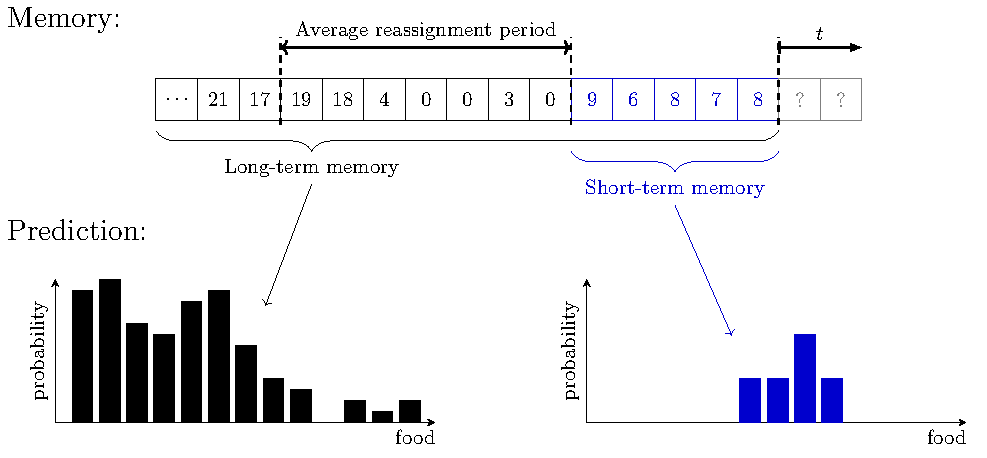
\includegraphics[width=0.9\linewidth]{008_team_6_agent_design/SOMAS_forecasting.pdf}
    \caption{Forecasting of the estimated food received in the short-term and long-term using two integer arrays.}
    \label{fig:forecasting}
\end{figure}

In order to distinguish between the short and long term, this agent also forecasts how long it will stay on the current floor. It does so by averaging the duration of previous reshuffling periods.

\subsection{Utility Theory}

Memory allows this agent to remember the past; Forecasting uses this to predict the future. In order to make a decision regarding treaties, one last step is required. Our agent needs to be able to compare two potential futures and decide which one it deems more beneficial. Behavioural research has shown that the utility a person gets gets from receiving something is not linear to the value of that thing and differs from. We thus use utility functions in our agents to model human decision making more accurately.\cite{fishburn1970utility}

Using utility functions, comparing which one of two different futures is more beneficial is simple. An agent calculates the expected utility with and without a treaty. It then maximise their estimated future benefit by choosing the larger expected utility.

Comparing potential future outcomes with utility allows us to introduce known psychological behaviours to our agents.

The expected utility of a gaining a certain amount of food $a$ is simply $E[U(a)] = U(a)$. The utility of gaining an uncertain amount of food resembled by the discrete random variable $x$ that is based on past experience, is computed given

\begin{equation} 
x = [ p_1: x_1, p_2: x_2; ... \;p_n: x_n]
\end{equation}

where an agent expects to get amount $x_i$ of food with probability $p_i$, such that

\begin{equation}
E[U(x)] = p_1 \times U(x_1) + p_2 \times U(x_2) + ... + p_n \times U(x_n)
\label{eq:expectedUtility}
\end{equation}

\subsubsection{\textit{Prospect Theory}}

Prospect theory, first established by Kahneman and Tversky in 1079, is a well established model of how we perceive a change in value, i.e. how much utility we get or loose out of a change in value. \cite{kahneman2013prospect}

\begin{figure} [h!]
    \centering
    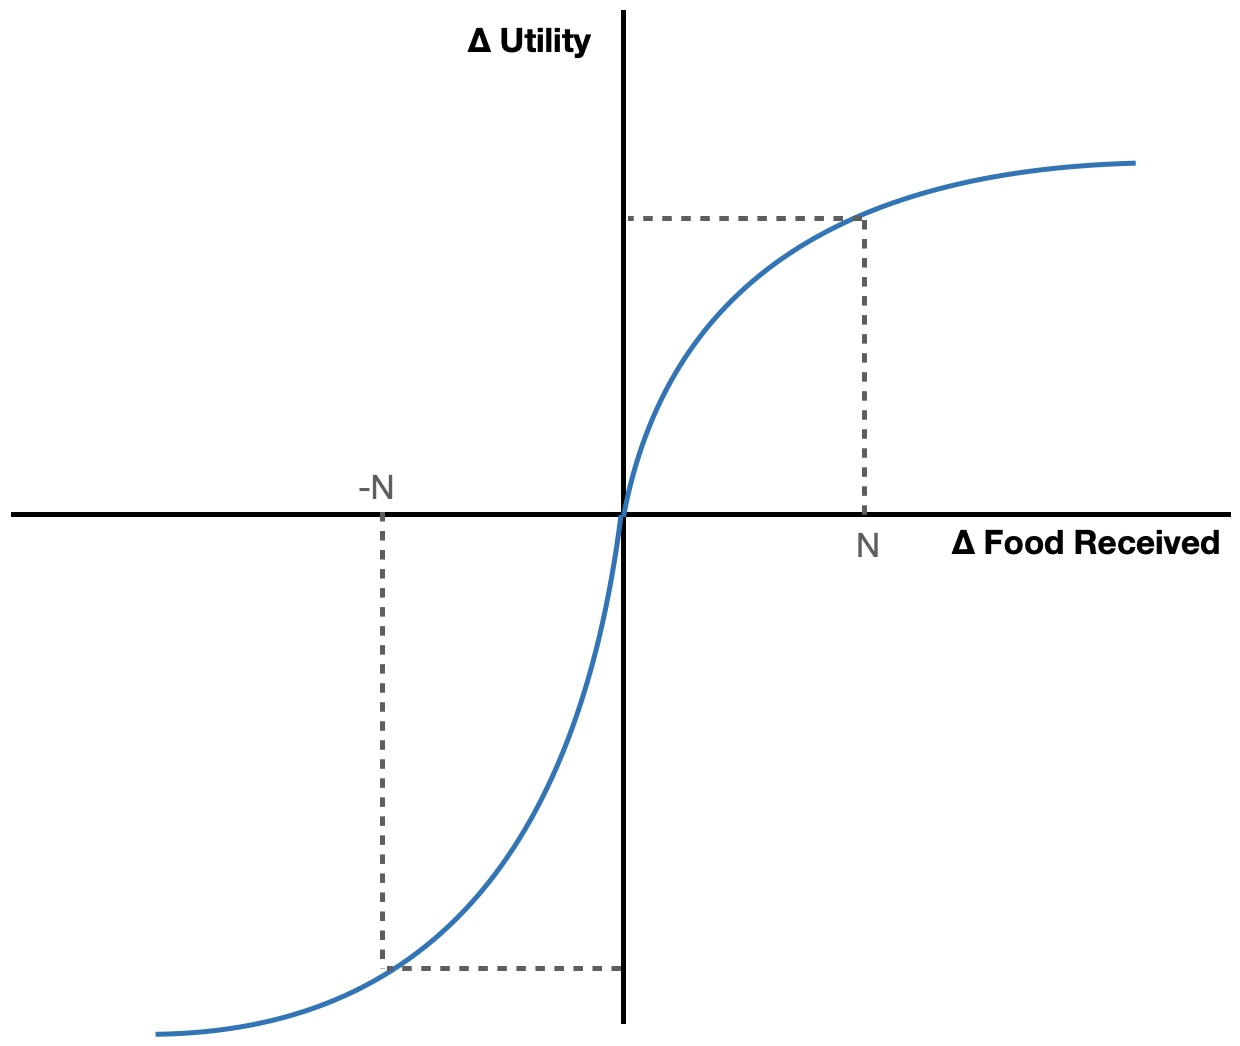
\includegraphics[width=0.5\linewidth]{008_team_6_agent_design/Prospect_Theory.jpg}
    \caption{Utility in decision making according to prospect theory.}
    \label{fig:prospect}
\end{figure}

Three main principles make up this model:
\begin{itemize}
    \item \textbf{Greediness:} Humans are generally greedy, i.e. more of something is always at least as beneficial to us. Utility functions hence are generally increasing \Cref{fig:prospect}.
    
    \item \textbf{Diminishing Sensitivity:} Marginal returns are strictly decreasing, i.e. the more we get, the less does one additional utility matter to us. An additional unit of food matters much more to our agents if it only gets one unit of food compared to if it gets 50 units of food.
    
    \item \textbf{Risk aversion:} Humans generally try to avoid risk. The discrete random distribution which forecasts the expected food received does not guarantee any certain amount of food and so is associated with risk. 
    With risk aversion, the amount of food our agent perceives as equivalent to a random distribution, its \textit{certainty equivalent} $C$, is hence less than its mean.

    \begin{equation}
    U(C) = E[U(x)] < U(E[x])    
    \end{equation}
    
    \item \textbf{Loss aversion:} Loosing some amount of food is generally perceived as worse than gaining that same amount. Our agents weigh loosing an amount of food stronger than gaining the same amount of food.
\end{itemize}

\subsection{Social Motives and Total Utility}

Prospect theory forms the basis to how we model our agents benefit from a change in consumption. However, in addition to the *gain,* there is also a *cost* that increases with eating more food: Every unit of food gained is one unit of food other agents lost. This social cost, combined with the previously explained explained utility, forms our total utility function. Each of our social motive corresponds to different values for greediness, risk-aversion, and social cost, which we have chosen according to three insights:

\begin{enumerate}
    \item The more selfish you are, the more greedy you are.
    
    \item The more you care for the greater good, the higher is your social cost associated with consumption.
    
    \item Studies such as the one by Campbell et al have shown that more narcissistic people are generally less risk-averse.
    \cite{campbell2004narcissism}
\end{enumerate}

We chose the parameters for each social motive accordingly, with greediness $g$, risk-seeking $r$ and social responsibility $c$, resulting in the total utility functions in \Cref{fig:utilities}.

\begin{itemize}
    \item \textbf{Altruist}: Not greedy, very risk-averse, very high social responsibility ($g=0 \: r=1 \: c=5$)
    
    \item \textbf{Collectivist}: a bit greedy, risk-averse, high social responsibility
    
    \item \textbf{Selfish}: greedy, little risk-aversion, little social responsibility
    
    \item \textbf{Narcissist}: very greedy, very little risk-aversion, no social cost
\end{itemize}

\ToDo{graphs for each utility function, parameters}
\label{fig:utilities}

\subsection{Weighing the Short- against the Long-Term}

As mentioned earlier, the futures our agent should expect in the short run (on the current level) and in the long run differ. The longer the duration of a treaty, the more should the long-term benefit matter. Using the short and long term memory of food received each day, our agent can separately estimate how much he will be getting on the floor he is currently on and how much he will be getting on average across all future reassignment periods.

By calculating the length of average reassignment period, our agents can estimate the number of days remaining on the current floor. We use the proportion of estimated days before the next reshuffling period to the duration of the treaty in order to weigh how much an agent should focus on the short term. Let $b_\text{short}$ and $b_\text{long}$ be the estimated long and short term benefit of a treaty, respectively. Also, let the estimated days remaining on the current level be given by $d_\text{current}$ and the duration of a treaty by $d_\text{treaty}$. The total benefit $b_\text{tot}$ is given by

\begin{equation}
b_\text{tot} = d\times b_\text{short} + (1-d)\times b_\text{long}    
\label{eq:shortlongweight}
\end{equation}

where $d = d_\text{current}/d_\text{treaty}$.

The following examples show how this plays out.

\begin{itemize}
    \item $d_\text{current} = 10$, $d_\text{treaty} = 8$:  $d=100\%$ (treaty expires before leaving the current floor)
    \item $d_\text{current} = 10$, $d_\text{treaty} = 20$: $d=50\%$
    \item $d_\text{current} = 10$, $d_\text{treaty} = 100$: $d = 10\%$
\end{itemize}


\subsubsection{\textit{Survival Instinct}}

When one is doing well, the above weighting between the long and short term benefits is sensible. However, if one is struggling to stay alive, survival instincts kick in. Consequently, our agents ignore the expected long-term utility all together when their health is on a critical level.

\subsection{Implementation}

How we rate treaties closely follows the theoretical steps from above. Every day, the agent stores the amount of food received in two arrays, one for the short-term and one for the long-term. The short-term array is reset after every reshuffling period. When a new treaty is proposed, our agent then...

\begin{enumerate}
    \item calculates what his expected short- and long-term utility is according to \Cref{eq:expectedUtility} and using the memory of food received in the past. The utility function used depends on their current social motive.
    \item amplifies the utility if it is negative in accordance to mimic loss-aversion.
    \item estimates the amount of food he can take under the treaty, i.e. the difference between the average amount of food he received in the past and the amount of much food he needs to leave in order to comply with the treaty, and calculate the utility of taking that amount of food.
    \item computes the estimated short-term and long-term benefit of signing the treaty as $U(\text{sign}) - U(\text{don’t sign})$.
    \item chooses to focus on the long-term or short-term benefit according to \Cref{eq:shortlongweight}
    \item signs the treaty if it’s overall benefit is positive
\end{enumerate}

The amount of food that the “collectivist” and “selfish” agents would need to consume in order to maximise utility varies depending on the current health level. The peak of their total utility function thus needs to be able to vary, too. We accounted for this by introducing a scaling factor $z$ without changing the general properties of the function, leading to:

\begin{equation}
U\left(x\right)=g\left(\frac{1}{z}\left(\frac{cr}{g}\right)^{\frac{r}{1-r}}x\right)^{\frac{1}{r}}-cx\frac{1}{z}\left(\frac{cr}{g}\right)^{\frac{r}{1-r}}    
\end{equation}
\subsection{Behaving according to treaties}

Treaties are fundamentally built on the assumption that all agents behave truthfully. Introducing dishonesty to treaties would strap them of all their power.

\ToDo{how do experimental results support this?}

Accordingly, we made sure that our agents behave in such a way as to never break any accepted treaty. 

This also means that our agents will never sign a treaty that contradicts previously accepted bounds on food intake.

\subsection{Proposing Treaties}
\ToDo{Describe how we propose treaties}


\newpage
%%%%%%%
%%%%%%% SIMULATION RESULTS
%%%%%%%
\section{Simulation Results and Discussion}\label{simulation_results}

%%
%% Hypothesis
%%
\subsection{Hypothesis}\label{hypothesis}
Before running presenting our simulation results, we present the hypothesis we want to verify. Knowing our modeling approach, the following main hypothesis and questions are relevant:
\begin{enumerate}

    \item In a purely narcissist system, it is impossible for an agent to survive on long-term.
    
    \item In a purely collectivist system, a stable state is reached instantaneously.
    
    \item In a system composed of agents with different social motives, a quasi-stable (\ToDo{define this term}) can be reached in  a long-term scenario.
    
        Show oscillation "period", also probably reflecting in the number of deaths per day and the utility per day
        
    \item There exist threshold on the number of selfish agents that can be incorporated in the system before a stable collectivist system becomes unstable.
     
     Experiment of Wednesday night with TakeFood treaties
     
    \item In a system composed of agents with different social motives, the use of treaties improve the global utility.
    
    try with vs without treaties on some configuration. for example with the experiment of point 4
    
    \item In a system composed of agents with different social motives, where genetic replacement of the agents occurs, The system converges to a collectivist system.
    
    implement genetic replacement
   
\end{enumerate}

%%
%% Summary of simulation
%%
\subsection{Summary of Simulations}\label{simulation_summary}

To examine the different hypothesis introduced in \Cref{hypothesis}, different simulations need to be performed. We divide our simulations into \ToDo{n} groups, each of them labelled by a capital letter (A, B, etc.) and having a different initialization procedure. \Cref{tab:simulation_summary} summarizes our simulations, together with their initial conditions. 

\begin{table}[htb]
    \centering
    \begin{tabular}{@{}lllll@{}}
    \toprule
    Name &  Behaviour initialization & maxBehaviour Swing & Stubbornness & special feature\\ \midrule
     A1              &  Altruist                    &  0 &    -     &  \\            
     A2              &  Collectivist                &  0 &     -    &  \\
     A3              &  Selfish                     & 0  &      -   &  \\       
     A4              &  Narcissist                  &  0 &      -   &  \\
     B1              &  Ratio 0.1,0.4,0.4,0.1       &  0 &    -     &  \\        
     B2              &  Ratio 0.55,0.7,0.2,0.05     &  0 &    -     & \\ 
     C1              &  Ratio 0.1,0.4,0.4,0.1       &  8 &    0.2   &    \\
     C2              &  Ratio 0.1,0.4,0.4,0.1       &  2 &    0.8   &    \\
     D1              &  Collectivist                &  6&      0.8& LeaveFoodTreaty       \\
     D2              &  Collectivist                &  6&    0.8  & TakeFoodTreaty I  \\
     D3              &  Collectivist                &  6 &    0.8 &  TakeFoodTreaty II \\
     E1              &  Ratio 0.25,0.25,0.25,0.25       &  6 &    0.2? &  Genetic Replacement I II\\
     E2              &  Ratio 0.25,0.25,0.25,0.25       &  4? &    0.2? &  Genetic Replacement\\\bottomrule
    \end{tabular}
    \caption{Summary of the simulations. \ToDo{Control parameters E1 and E2.}}
    \label{tab:simulation_summary}
\end{table}

Genetic Replacement I: 100 Agents, 50 Food, 100 MaxHP, 60 Days

Genetic Replacement II: : 100 Agents, 500 Food, 100 MaxHP, 60 Days

\ToDo{Explain the initialization parameters \textbf{@Matt Scott?}}

\ToDo{Make the table look good}

%%
%% Simulation Results
%%
\subsection{Simulation Results and Discussion}

In this section, we present the results by simulating our system according to \Cref{tab:simulation_summary}.


%%%
\subsubsection{Simulations A: Single Agent Type}

 The results are shown in \Cref{fig:res_A}.

\begin{figure}[htb]
    \centering
    \begin{tabular}{cc}
    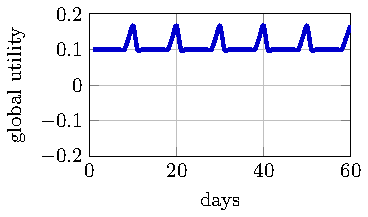
\includegraphics[width=0.3\linewidth]{008_team_6_agent_design/A/SOMAS_A1_utility.pdf} &   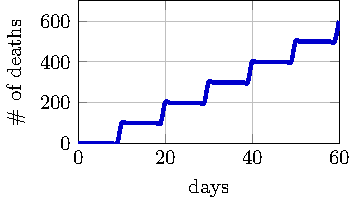
\includegraphics[width=0.3\linewidth]{008_team_6_agent_design/A/SOMAS_A1_deaths.pdf} \\[0pt]
    (a) A1: utility over time & (b) A1: deaths over time \\[8pt]
     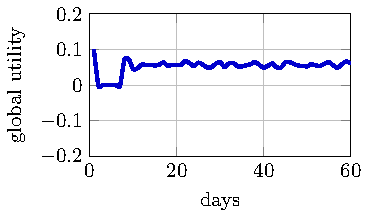
\includegraphics[width=0.3\linewidth]{008_team_6_agent_design/A/SOMAS_A2_utility.pdf} &   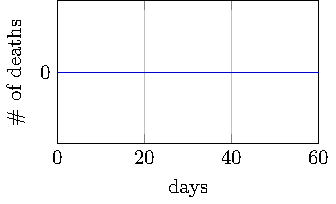
\includegraphics[width=0.3\linewidth]{008_team_6_agent_design/A/SOMAS_A2_deaths.pdf} \\[0pt]
    (c) A2: utility over time & (d) A2: deaths over time
    \\[8pt]
     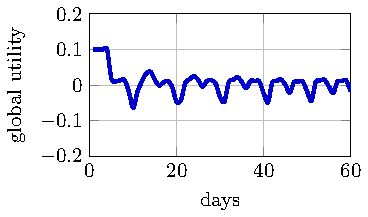
\includegraphics[width=0.3\linewidth]{008_team_6_agent_design/A/SOMAS_A3_utility.pdf} &   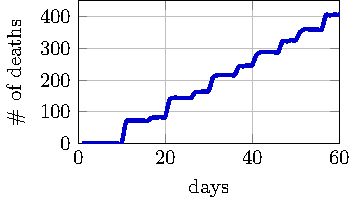
\includegraphics[width=0.3\linewidth]{008_team_6_agent_design/A/SOMAS_A3_deaths.pdf} \\[0pt]
    (e) A3: utility over time & (f) A3: deaths over time
    \\[8pt]
     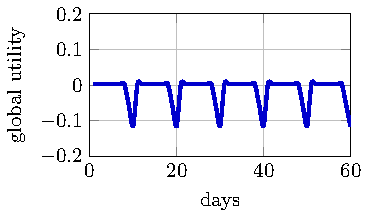
\includegraphics[width=0.3\linewidth]{008_team_6_agent_design/A/SOMAS_A4_utility.pdf} &   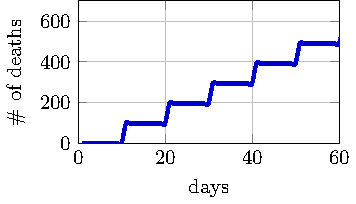
\includegraphics[width=0.3\linewidth]{008_team_6_agent_design/A/SOMAS_A4_deaths.pdf} \\[0pt]
    (g) A4: utility over time & (h) 4: deaths over time
    \end{tabular}
    \caption{Simulation results for a group of agents with uniform social motive.}
    \label{fig:res_A}%
\end{figure}

%%%
\subsubsection{Simulations B: Multiple Agent Types without Behaviour Change}

\ToDo{to simulate and add: utility over time, death over time}

%%%
\subsubsection{Simulations C: Multiple Agent Types with Behaviour Change}

\ToDo{to simulate and add: utility over time, death over time}

%%%
\subsubsection{Simulations D: Destabilization of a Collectivist System}
 The results are shown in \Cref{fig:res_D}.
 
\ToDo{Add results D3}

\begin{figure}[htb]
    \centering
    \begin{tabular}{ccc}
    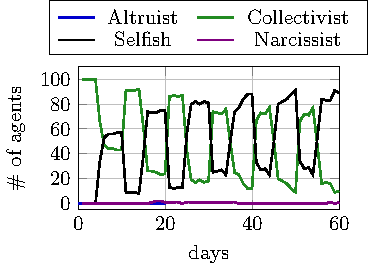
\includegraphics[width=0.3\linewidth]{008_team_6_agent_design/D/D1_SM.pdf} &   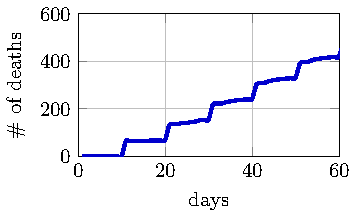
\includegraphics[width=0.3\linewidth]{008_team_6_agent_design/D/D1_deaths.pdf} &
    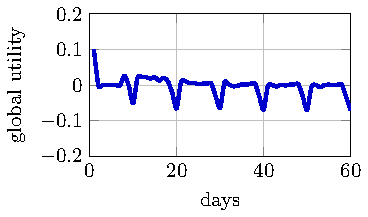
\includegraphics[width=0.3\linewidth]{008_team_6_agent_design/D/D1_utility.pdf}\\[0pt]
    (a) D1: social motives & (b) D1: deaths over time & (c) D1: utility over time \\[8pt]
         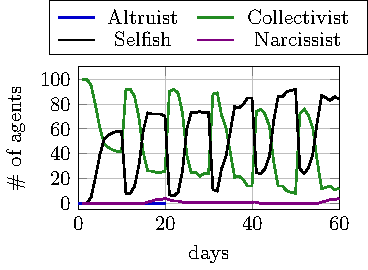
\includegraphics[width=0.3\linewidth]{008_team_6_agent_design/D/D2_SM.pdf} &   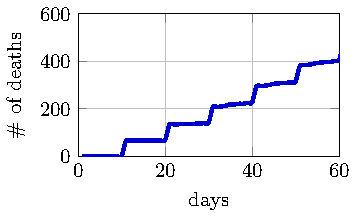
\includegraphics[width=0.3\linewidth]{008_team_6_agent_design/D/D2_deaths.pdf} &
    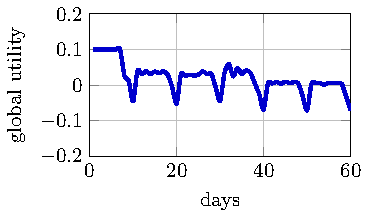
\includegraphics[width=0.3\linewidth]{008_team_6_agent_design/D/D2_utility.pdf}\\[0pt]
    (d) D2: social motives & (e) D2: deaths over time & (f) D2: utility over time \\[8pt]
    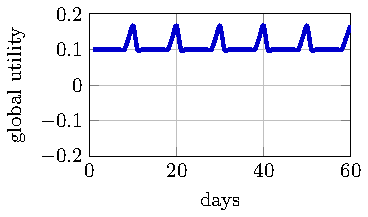
\includegraphics[width=0.3\linewidth]{008_team_6_agent_design/A/SOMAS_A1_utility.pdf} &   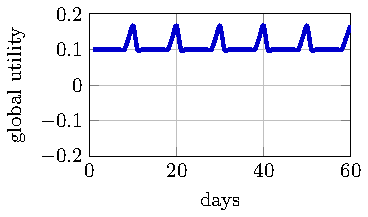
\includegraphics[width=0.3\linewidth]{008_team_6_agent_design/A/SOMAS_A1_utility.pdf} &
    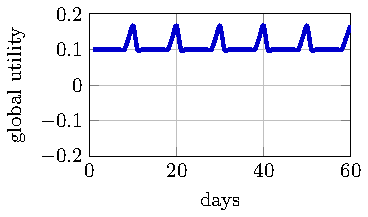
\includegraphics[width=0.3\linewidth]{008_team_6_agent_design/A/SOMAS_A1_utility.pdf}\\[0pt]
    (g) D3: social motives & (h) D3: deaths over time & (i) D3: utility over time \\[8pt]
    \end{tabular}
    \caption{Simulation results different treaties acceptances.}
    \label{fig:res_D}%
\end{figure}

%%%
\subsubsection{Simulations E: Genetic Replacement of Agents}

 The results are shown in \Cref{fig:res_E}.

\ToDo{Add results E2}

\begin{figure}[htb]
    \centering
    \begin{tabular}{ccc}
    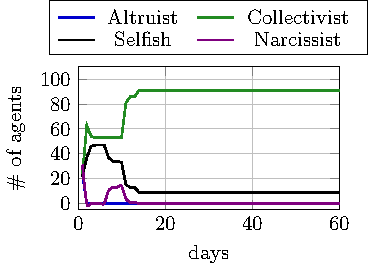
\includegraphics[width=0.3\linewidth]{008_team_6_agent_design/E/E1_SM.pdf} &   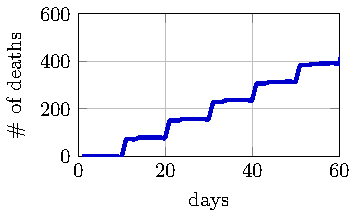
\includegraphics[width=0.3\linewidth]{008_team_6_agent_design/E/E1_deaths.pdf} &
    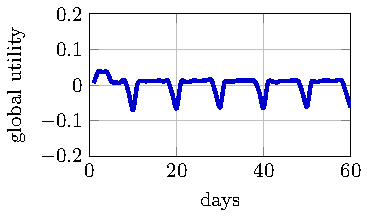
\includegraphics[width=0.3\linewidth]{008_team_6_agent_design/E/E1_utility.pdf}\\[0pt]
    (a) D1: social motives & (b) D1: deaths over time & (c) D1: utility over time \\[8pt]
         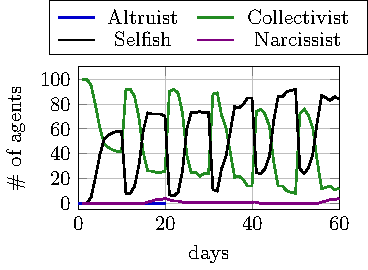
\includegraphics[width=0.3\linewidth]{008_team_6_agent_design/D/D2_SM.pdf} &   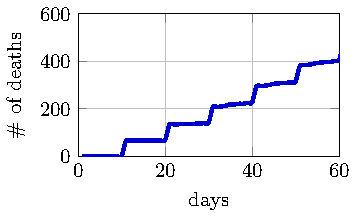
\includegraphics[width=0.3\linewidth]{008_team_6_agent_design/D/D2_deaths.pdf} &
    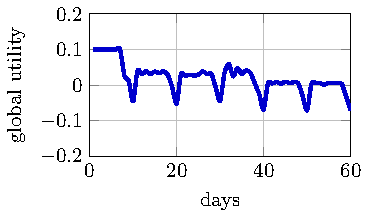
\includegraphics[width=0.3\linewidth]{008_team_6_agent_design/D/D2_utility.pdf}\\[0pt]
    (d) D2: social motives & (e) D2: deaths over time & (f) D2: utility over time 
    \end{tabular}
    \caption{Simulation results with genetic replacement of the agents.}
    \label{fig:res_E}%
\end{figure}
